\documentclass{article}
\usepackage{amsmath}
\usepackage[legalpaper, margin=0.5in]{geometry}
\usepackage[final]{pdfpages}

\title{Elliptic Curve Exercises}
\author{Cecilia Chan}

\begin{document}
\maketitle

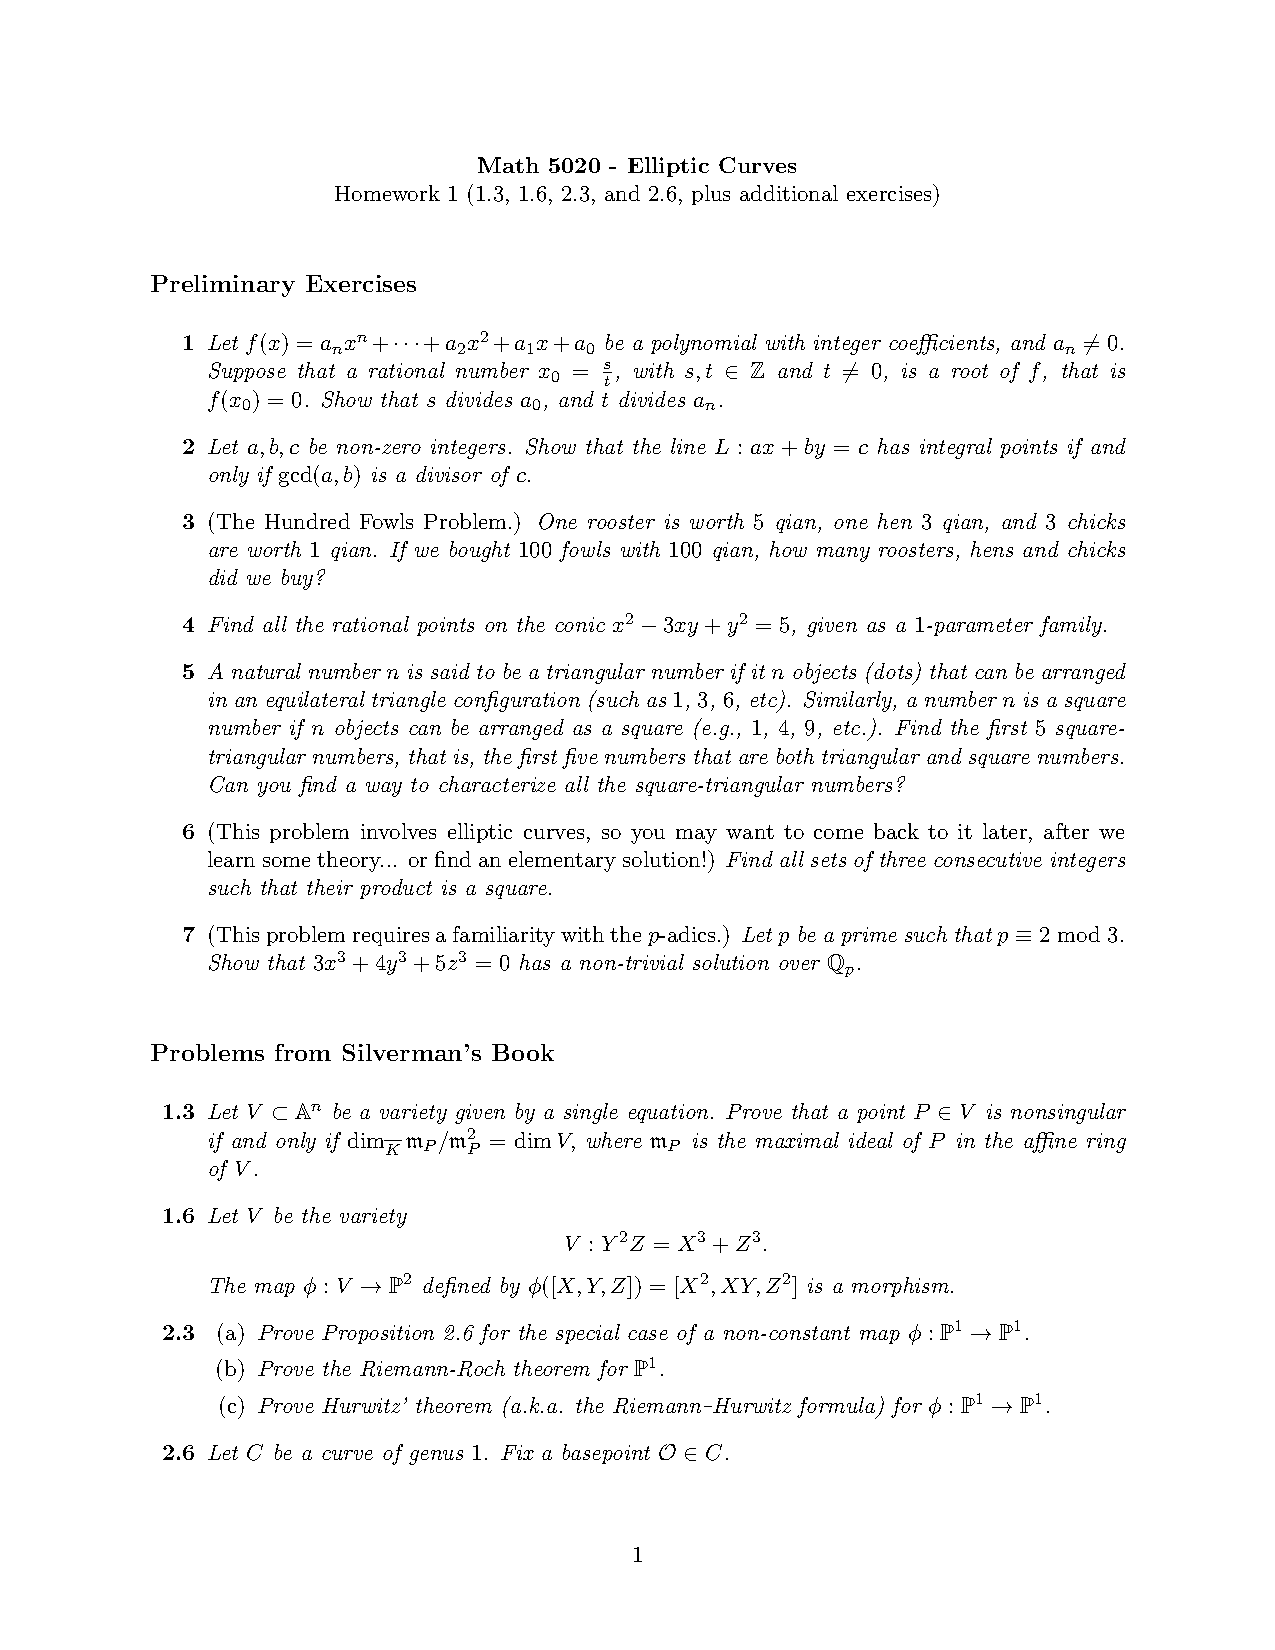
\includepdf{Misc/Elliptic/MATH-5020-hw1-1.pdf}

\section*{Problem 1}
Consider:
\begin{eqnarray*}
  a_0 + \sum\limits_{i = 1}^{n} a_i \left(\frac{s}{t}\right)^i &=& 0                                     \\
            a_0 t^n  + \sum\limits_{i = 1}^{n} a_i s^i t^{n-i} &=& 0                                     \\
                                                   a_0 t^n &=& - \sum\limits_{i = 1}^{n} a_i s^i t^{n-i}
\end{eqnarray*}
Note that every term of the right hand size is a multiple of $ s $, but $ \gcd(s^n, t) = \gcd(s, t) = 1 $, so $ a_0 $ is a multiple of $ s $.

Consider:
\begin{eqnarray*}
  \sum\limits_{i = 0}^{n-1} a_i \left(\frac{s}{t}\right)^i + a_n \left(\frac{s}{t}\right)^n &=& 0 \\
  \sum\limits_{i = 0}^{n-1}  a_i s^i t^{n-i} + a_n s^n &=& 0 \\
  a_n s^n &=& -\sum\limits_{i = 0}^{n-1} a_i s^i t^{n-i}
\end{eqnarray*}
Note that every term on the right hand side is a multiple of $ t $, but $ \gcd(s^n, t) = \gcd(s, t) = 1 $, so $ a_n $ is a multiple of $ t $.

\section*{Problem 2}
$ \Rightarrow $:

Suppose $ ax + by = c $ has integral solution $ (x, y) $, then $ \frac{a}{\gcd(a, b)} x + \frac{b}{\gcd(a, b)} y = \frac{c}{\gcd(a, b)} $. In this case, left hand side is an integer, so is the right hand side, and therefore $ c $ is a multiple of $ \gcd(a, b) $.

$ \Leftarrow $:

Suppose $ c $ is a multiple of $ \gcd(a, b) $, then $ c = k \gcd(a, b) $ for some integer $ k $. By Bezout's identity, there exists $ x_0, y_0 $ such that $ ax_0 + by_0 = \gcd(a, b) $. Then $ a(kx_0) + b(ky_0) = c $, and $ (kx_0, ky_0) $ is an integral solution to $ ax + by = c $.

\section*{Problem 3}
Let the number of rooster, hen and chicken be $ r, h, c $ respectively. Then we have:

\begin{eqnarray*}
  r + h + c &=& 100 \\
  5r + 3h + \frac{1}{3}c &=& 100
\end{eqnarray*}

To avoid fraction, we can have:
\begin{eqnarray*}
  r + h + 3d &=& 100 \\
  5r + 3h + d &=& 100
\end{eqnarray*}

Or in matrix form 

\begin{eqnarray*}
  A &=& \left(
  \begin{array}{ccc}
    1 & 1 & 3 \\
    5 & 3 & 1 
  \end{array}\right) \\
  b &=& \left(\begin{array}{c}
    r \\
    h \\
    d
  \end{array}\right) \\
  b &=& \left(\begin{array}{c}
    100 \\
    100
  \end{array}\right) \\
  Ax &=& b
\end{eqnarray*}

Smith normal form allow us to write $ A = P^{-1} S Q^{-1} $ where $ P, Q $ are unimodular matrices, and $ S $ is a diagonal matrix.

\begin{eqnarray*}
  P &=& \left(
  \begin{array}{cc}
    1 & 0 \\
    5 & -1
  \end{array}\right) \\
  Q &=& \left(
  \begin{array}{ccc}
    1 & -1 & 4 \\
    0 & 1 & -7 \\
    0 & 0 & 1
  \end{array}\right) \\
  S &=& \left(
  \begin{array}{ccc}
    1 & 0 & 0 \\
    0 & 2 & 0 \\
  \end{array}\right) \\
\end{eqnarray*}

Now we can easily solve the system as follows:
\begin{eqnarray*}
  Ax &=& b \\
  P^{-1} S Q^{-1} x &=& b \\
  S Q^{-1} x &=& P b \\
  \left(
  \begin{array}{ccc}
    1 & 0 & 0 \\
    0 & 2 & 0 \\
  \end{array}\right) Q^{-1}x &=& \left(\begin{array}{c}
               100 \\
               400 
              \end{array}\right) \\
              Q^{-1}x &=& \left(\begin{array}{c}
               100 \\
               200 \\
               t
              \end{array}\right) \\
  x &=& Q \left(\begin{array}{c}
               100 \\
               200 \\
               t
              \end{array}\right) \\
  x &=& \left(
    \begin{array}{ccc}
      1 & -1 & 4 \\
      0 &  1 & -7 \\
      0 & 0 & 1 
    \end{array}\right) \left(\begin{array}{c}
      100 \\
      200 \\
      t
     \end{array}\right) \\
  \left(\begin{array}{c}
    r \\
    h \\
    d
  \end{array}\right) &=& \left(\begin{array}{c}
    4t - 100 \\
    -7t + 200 \\
    t
  \end{array}\right)
\end{eqnarray*}

All of these are number of animals, so it must be the case that they are non-negative. Therefore we have:
\begin{eqnarray*}
   4t - 100 &\geq& 0 \\
          t &\geq& 25 \\
  -7t + 200 &\geq& 0 \\
          t &\leq& \frac{200}{7} \\
          t &\leq& 28 \\
\end{eqnarray*}

So the answer is obvious, $ t $ can only be $ 25, 26, 27, 28 $, and the corresponding number of rooster, hen and chicken are $ 0, 25, 75 $, $ 4, 18, 78 $, $ 8, 11, 81 $, $ 12, 4, 84 $ respectively.

\end{document}